\section{Method}
A controlled trial was designed, whereby the subjects were randomly, but with an equal gender distribution, assigned into a control and treatment group, as illustrated on \autoref{fig:studydesign}.
%******COMMENT*****say something about blind TOBY?? - I think it would be better when we mention under the experimental procedure section.
\begin{figure}[H]
\centering
%\caption{} \vspace{-.25cm}
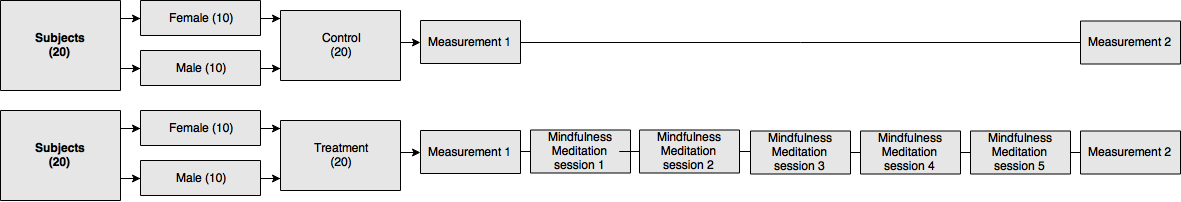
\includegraphics[width=1\columnwidth]{../figures/studydesign.png}
\caption{Study design}
\label{fig:studydesign}
\end{figure} \vspace{-.5cm}


\subsection{Subjects}
44 healthy subjects, 20 men and 24 women were recruited(age: 2X$\pm$XX years and BMI: XX$\pm$XX). 
%*****COMMENT**** we need no say the BMI??
Subjects with ongoing meditation practice, acute or chronic pain, neurological, musculoskeletal or mental illness, pregnancy or medications that might influence the subjects’ response to pain were excluded.

\subsection{Experimental Procedure}
Testing points, as seen on \autoref{fig:trapezius}, were marked at the right upper trapezius (UT) to ensure reliable and rapid location during the experimental procedure. The location of the upper trapezius was determined between the acromion and 7th cervical vertebra. The baseline values of Pressure Pain Threshold and Pressure Pain Tolerance were measured with an algometer (Wagner Force Ten™ Digital force Gage) three times. The examiner was blinded during the three measurements to avoid bias. The mean of three measurements, was computed. 

\begin{figure}[H]
\centering
%\caption{} \vspace{-.25cm}
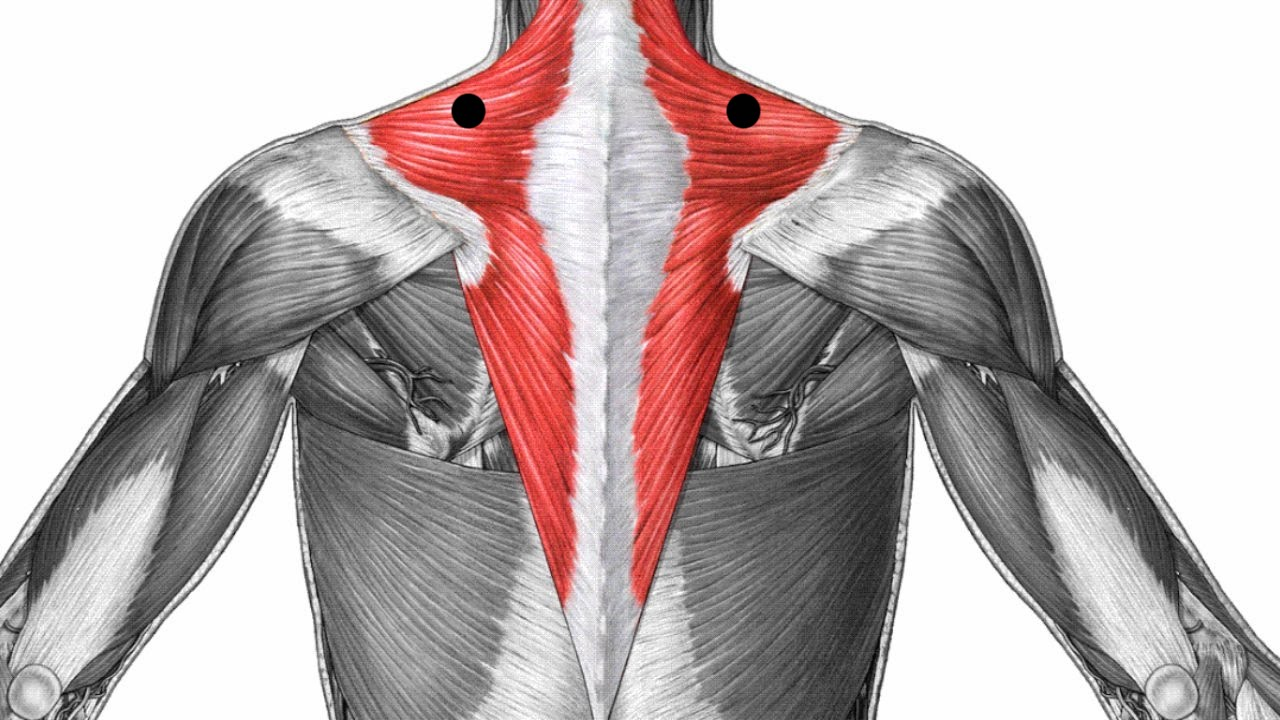
\includegraphics[width=.7\columnwidth]{../figures/trapezius}
\caption{Testing points on the upper trapezius.}
\label{fig:trapezius}
\end{figure} \vspace{-.5cm}

The treatment group practiced 20 minutes mindfulness meditation on 5 consecutive days. After the last meditation session the second measurement was conducted likewise the baseline measurement.
The subjects of the control group continued their normal routine. The same time interval between baseline and second measurement was used for the subjects of the control group.

\subsection{Meditation Technique}
Short-term mindfulness meditation with 20 minutes of meditation on 5 consecutive days.
To ensure same meditation conditions, a guided meditation in form of an audio file was used. A short introduction to mindfulness meditation was provided before the first meditation session. The meditation was focused attention focusing on breath flow.
Here / In this section is missing a little bit! Maybe about FA

\subsection{Data Analysis}
To test the effect of mindfulness meditation on chronic neck pain, a paired t-test / Mann-Whitney / Wilcoxon rank test was applied to the baseline and second measurement of both groups, the treatment and the control group.
